\chapter{Mimicking Non-Monotonic Logics With SCPs} \label{chp:mimick}

\section{The Suppression Task}

\section{The Weak Completion Semantics}



\chapter{Modelling Experiments with SCPs} \label{chp:model}
\section{Overview}
As with any cognitive framework, the most important metric for judging the success of SCPs comes from testing how well SCPs can approximate empirical data across tasks. This chapter will show the suitability of SCPs with a common set of allowable cognitive operations for modelling several well-studied experiments in cognitive modelling.

In particular, we will show that the Wason Selection Task, Suppression Task and @TODO can be modelled at both the general and individual reasoner level with SCPs in a formulation that intuitive and consistent with the WCS approach already described in Section~@TODOref.
\section{Suppression Task}

\begin{figure*}
\begin{center}
 \centering 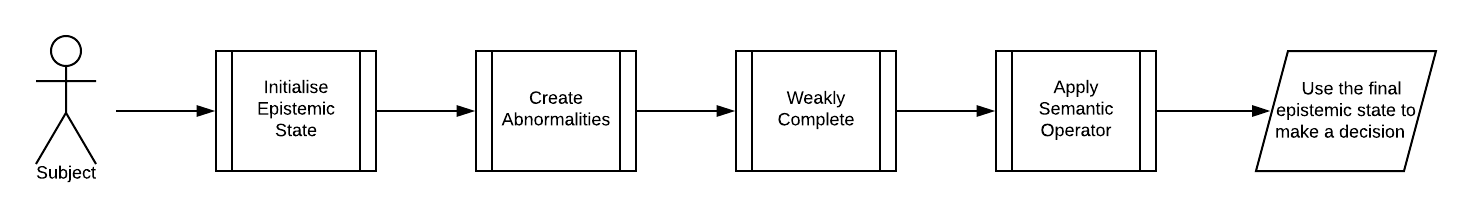
\includegraphics[width=\linewidth]{suppressionSCP_overview}
\caption{A generalised illustration of the WCS in an SCP. }
\label {fig:supoverview}
\end{center}
\end{figure*}

\begin{figure*}
\begin{center}
 \centering 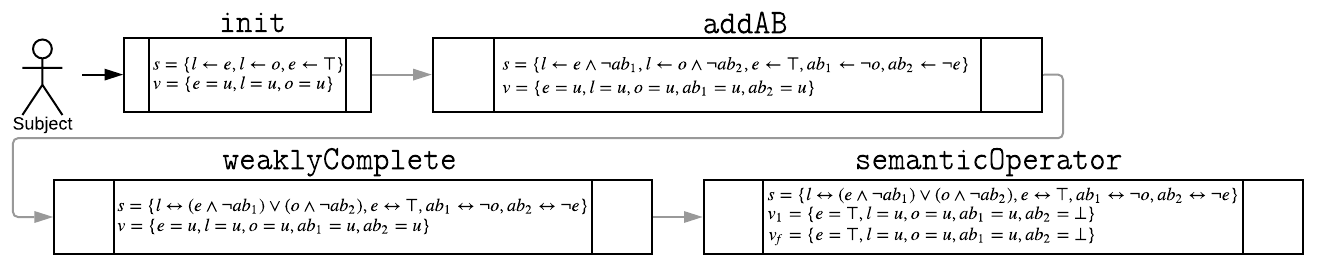
\includegraphics[width=\linewidth]{suppressionSCP_normal}
\caption{The standard case of the Suppression Task, demonstrating the suppression effect. Where the epistemic state in the boxes represents the output of that cognitive operation. $V_f$ represents the assignment of $V$ in the epistemic state in the resulting least model. $V_{i\in \mathbb{N}}$ represents the assignments in $V$ after $i$ iterations of the semantic operator.}
\label {fig:supnormal}
\end{center}
\end{figure*}

Figure~\ref{fig:supoverview} illustrates a generalised SCP to describe the Suppression Task as a series of sequential steps directly mirroring the discrete steps outlined in Section~\ref{sec:sup}, each cognitive operation passing information to the next process\footnote{It is important to note that a diagram like this is valid for \textit{any} cognitive modelling task because any process may be arbitrarily complex and non-sequential. and so the overall linear process of (actor, complex decision, observed results) is always valid for retroactive modelling, and at least as powerful as the non-monotonic logic framework it uses for modelling.}. To model the SCP the implicit sequence of operations in the Suppression Task is systematized and refined into a set of complex operations. Further we introduce an initial epistemic state $s_i=(KB,V,R)$. One interpretation of the requirements of the suppression task $\pi=(s_i,\gamma,M)$ using SCPs and the WCS is as follows: 
 
 
 
 


\[s_i=\{KB_i, V_i, R_i\} \]
\[KB_i=\{e \rightarrow l, \top \rightarrow e, o \rightarrow l\} \]
\[V_i=\{e:u, l:u, o:u\} \]
\[R_i=\{\} \]
\[
\begin{split}
M= \{\texttt{init}, \texttt{addAB}, \texttt{WeaklyComplete}, \texttt{semanticOperator}\}
\end{split}
\]
\[\gamma = (l\models \top) \textrm{ or } (l \models \bot)\]

%@TODO change semanticOper to semanticOperator without line overflowing 

where all cognitive operations require as input and produce as output a state point $p$ where every ground point $\bar{p} \in_s p$ is of format $\bar{p}=(KB,V,R)$; \texttt{init} is always the first cognitive operation and adds the initial variables and rules to epistemic state; \texttt{addAB} adds abnormalities to the current epistemic state using the procedure described in Algorithm~\ref{alg:addAbnormalities} (but now also adds those abnormalities to the variable list of the epistemic state); \texttt{WeaklyComplete} weakly completes the knowledge base of the current epistemic state; and \texttt{semanticOperator} returns an epistemic state that leaves the knowledge base unchanged but updates the variables of that state to return the least model of the epistemic state. \texttt{semanticOperator} follows the same logic seen in Section~\ref{ssec:wcs}, but directly updating $V$ after each iteration of the semantic operator, instead of the externalised variable set $J$. Thus, we ensure that the output state point is able to communicate the result of applying the semantic operator without any structural changes to the epistemic states it contains. As an additional feature of the \texttt{semanticOperator} cognitive operation, if there exists a labelled set in $R$ called $fixed$, then the semantic operator will not set the value of any $v \in fixed$ in the variables list $V$. The goal $\gamma$ states that $l$ should no longer be mapped to unknown in the final epistemic state.



Treating Figure~\ref{fig:supoverview} as an SCP, we observe the sequence of output states seen in Figure~\ref{fig:supnormal}. Note that in the final state $l$ remains mapped to $u$, meaning that the suppression effect is demonstrated.

\subsection{Extending the Suppression Task with SCPs}
The previous example merely showed that SCPs are suitable for modelling the suppression task. In this example we consider one of the most powerful characteristics of SCPs, the ability to model unusual results as deviations from general reasoning. In the original Suppression Task Experiment examined in Section~\ref{sec:sup}, a significant portion of people still believed that she would study late in the library, even though the majority suppressed the inference. Several possible explanations are intuitive, the first and simplest, is the assumption that the reasoner is using classical logic and drawing the classical conclusion. However, what if that is not the case? What if they do reason in exactly the same way as the other reasoners, except for one or two small deviations?

In order to model these non-general reasoners, we consider two possible deviations that could explain the classical result of the Suppression Task: \textit{variable deletion}, and\textit{ variable fixation}. Both of these operations will be discussed in a way that may seem overly prosaic, but it is done to reinforce that we might, reasonably, expect these cognitive operations to occur in day-to-day human cognition.


\begin{figure*}
\begin{center}
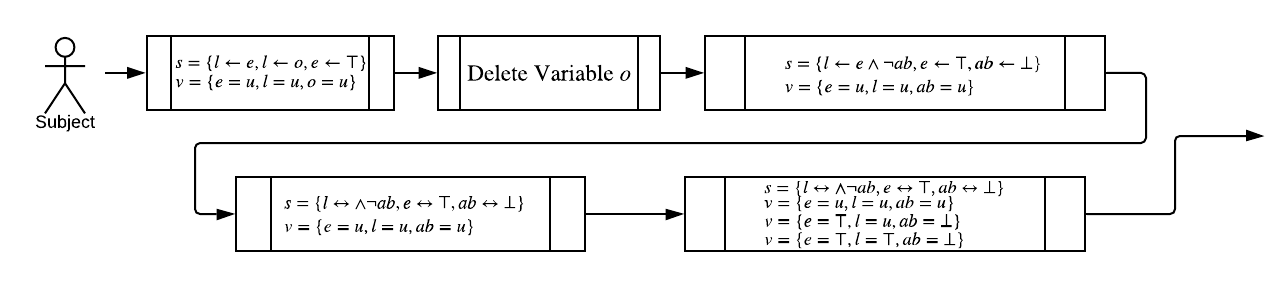
\includegraphics[width=0.85\linewidth]{suppressionSCP_mod}
\end{center}

\caption{The Suppression Task in which the additional operation of deleting the variable $o$ occurs.}
\label{fig:supmod}
\end{figure*}

\begin{figure*}
\begin{center}
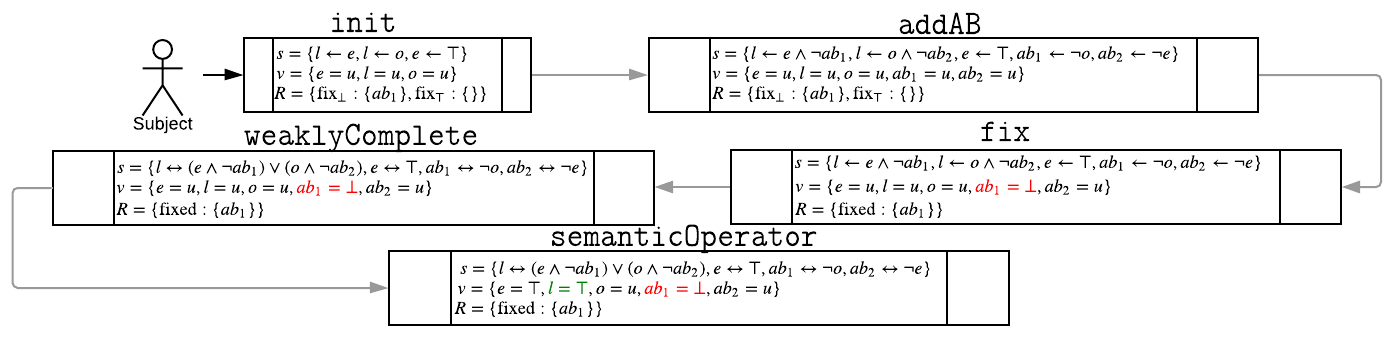
\includegraphics[width=\linewidth]{suppressionSCP_mod2}
\end{center}

\caption{The Suppression Task in which the additional operation of fixing the variable $ab_1$ to false occurs.}
\label{fig:supmod2}
\end{figure*}
\section{Wason Selection Task}

\[\Pi=(s_i,M,f(),\gamma\]



\[\mu=(\pi,f())\]

The choice of external evaluation function for this task (the turn function), if we are to follow the intuition from @TODO, has two requirements: it must be able to capture whether an observation $O$ can be explained by the least model of the weakly completed program, and it must ensure that variable assignments which,if incorrect could falsify the rule $2\leftarrow D$, are present in the least model. To this end, we add an observation variable $O$ to the definition of the initial epistemic state, and combine this with the variables for the set of propositional rules $S$, conditional rules $\Delta$, and possible world $V$.



\[f(\pi,O)==  I_V(O)\models \top \textrm{ and } I_V(D)\models \top \lor \bot \textrm{ and } I_V(3)\models \top \lor \bot\]



Next, we require an intuition for the generation of the initial epistemic state point $s_i$. In this case, abduction can be simulated by the SCP in one of three ways. The first is to create a unique SCP for each possible explanation for each observation as we did for the classical WCS interpretation of the task in Section~@TODOref. But the fact that SCPs may contain an initial state point, rather than just a single epistemic state, enables a more elegant solution that captures the full scope of possible observation, explanation pairings. The other two options are to start with a state point containing each abductive case, or to create cognitive operations which create these abductive cases at computation time.

Because SCPs aim to capture as much cognitive information as possible within the CTM as possible, we will prefer this third case and make use of a categorization variable $R$ to specify both the set of observations $O$, and the possible explanations $\eta$. The cognitive operation \texttt{AddExp} is created.

\texttt{AddExp} adds possible explanations $\eta$ to the set of rules $S$ in the epistemic state and is defined as follows:

%------
\[\texttt{AddExp}(\textit{input})=(\chi,e)\]
\[\chi=(\textit{input}\models (S,R))\]
\[e=\]
\[R'\subseteq R[\textrm{'explanations'}]\]
\[d := (R'[1]\cup...\cup R'[n])\]

\[S:=S\cup d\]

\[R[\epsilon]:=R[\epsilon] \cup e\]
@TODOdefine$\cup$forR
%------

Figure~@TODOref shows the state point that results from applying this cognitive operation to $s_i=(S=\{\},\Delta=\{(3|D)\},V=\{D,K,3,7\},O=\{\},R=\{'explanations':\{D,K,3,7\}\})$ for cases where $R'$ is a single abducible.

Because the intention of this task is model a known response set for the WST, we must consider some way of generating an SCP in which $f(\pi)= \gamma$. As before this necessitates an appropriate selection of cognitive functions for $M$. We will make use of the set:

\[
M=\{\texttt{addAB},\texttt{wc},\texttt{semantic}, \texttt{addExp}\}
\]

Conducting de Novo search on $\Pi$ for each of the observations at this point now returns a state point containing the following CTMs:
\[
\pi_1=(s_i \longmapsto \texttt{addAB} \texttt{addExp} \longmapsto \longmapsto \texttt{wc} \longmapsto \texttt{semantic}))
\]

\[
\pi_2=(s_i \longmapsto \texttt{addExp} \longmapsto \texttt{addAB} \longmapsto \texttt{wc} \longmapsto \texttt{semantic}))
\]


\[
\mu_D^1=(\pi_1), f(\pi, O=\{D\}))
\]
\[
\mu_D^2=(\pi_2), f(\pi, O=\{D\}))
\]

\[
\mu_K^1=(\pi_1), f(\pi, O=\{K\}))
\]
\[
\mu_K^2=(\pi_2), f(\pi, O=\{K\}))
\]

\[
\mu_3^1=(\pi_1), f(\pi, O=\{3\}))
\]
\[
\mu_3^2=(\pi_2), f(\pi, O=\{3\}))
\]

\[
\mu_7^1=(\pi_1), f(\pi, O=\{7\}))
\]
\[
\mu_7^2=(\pi_2), f(\pi, O=\{7\}))
\]

\begin{figure}
\centering{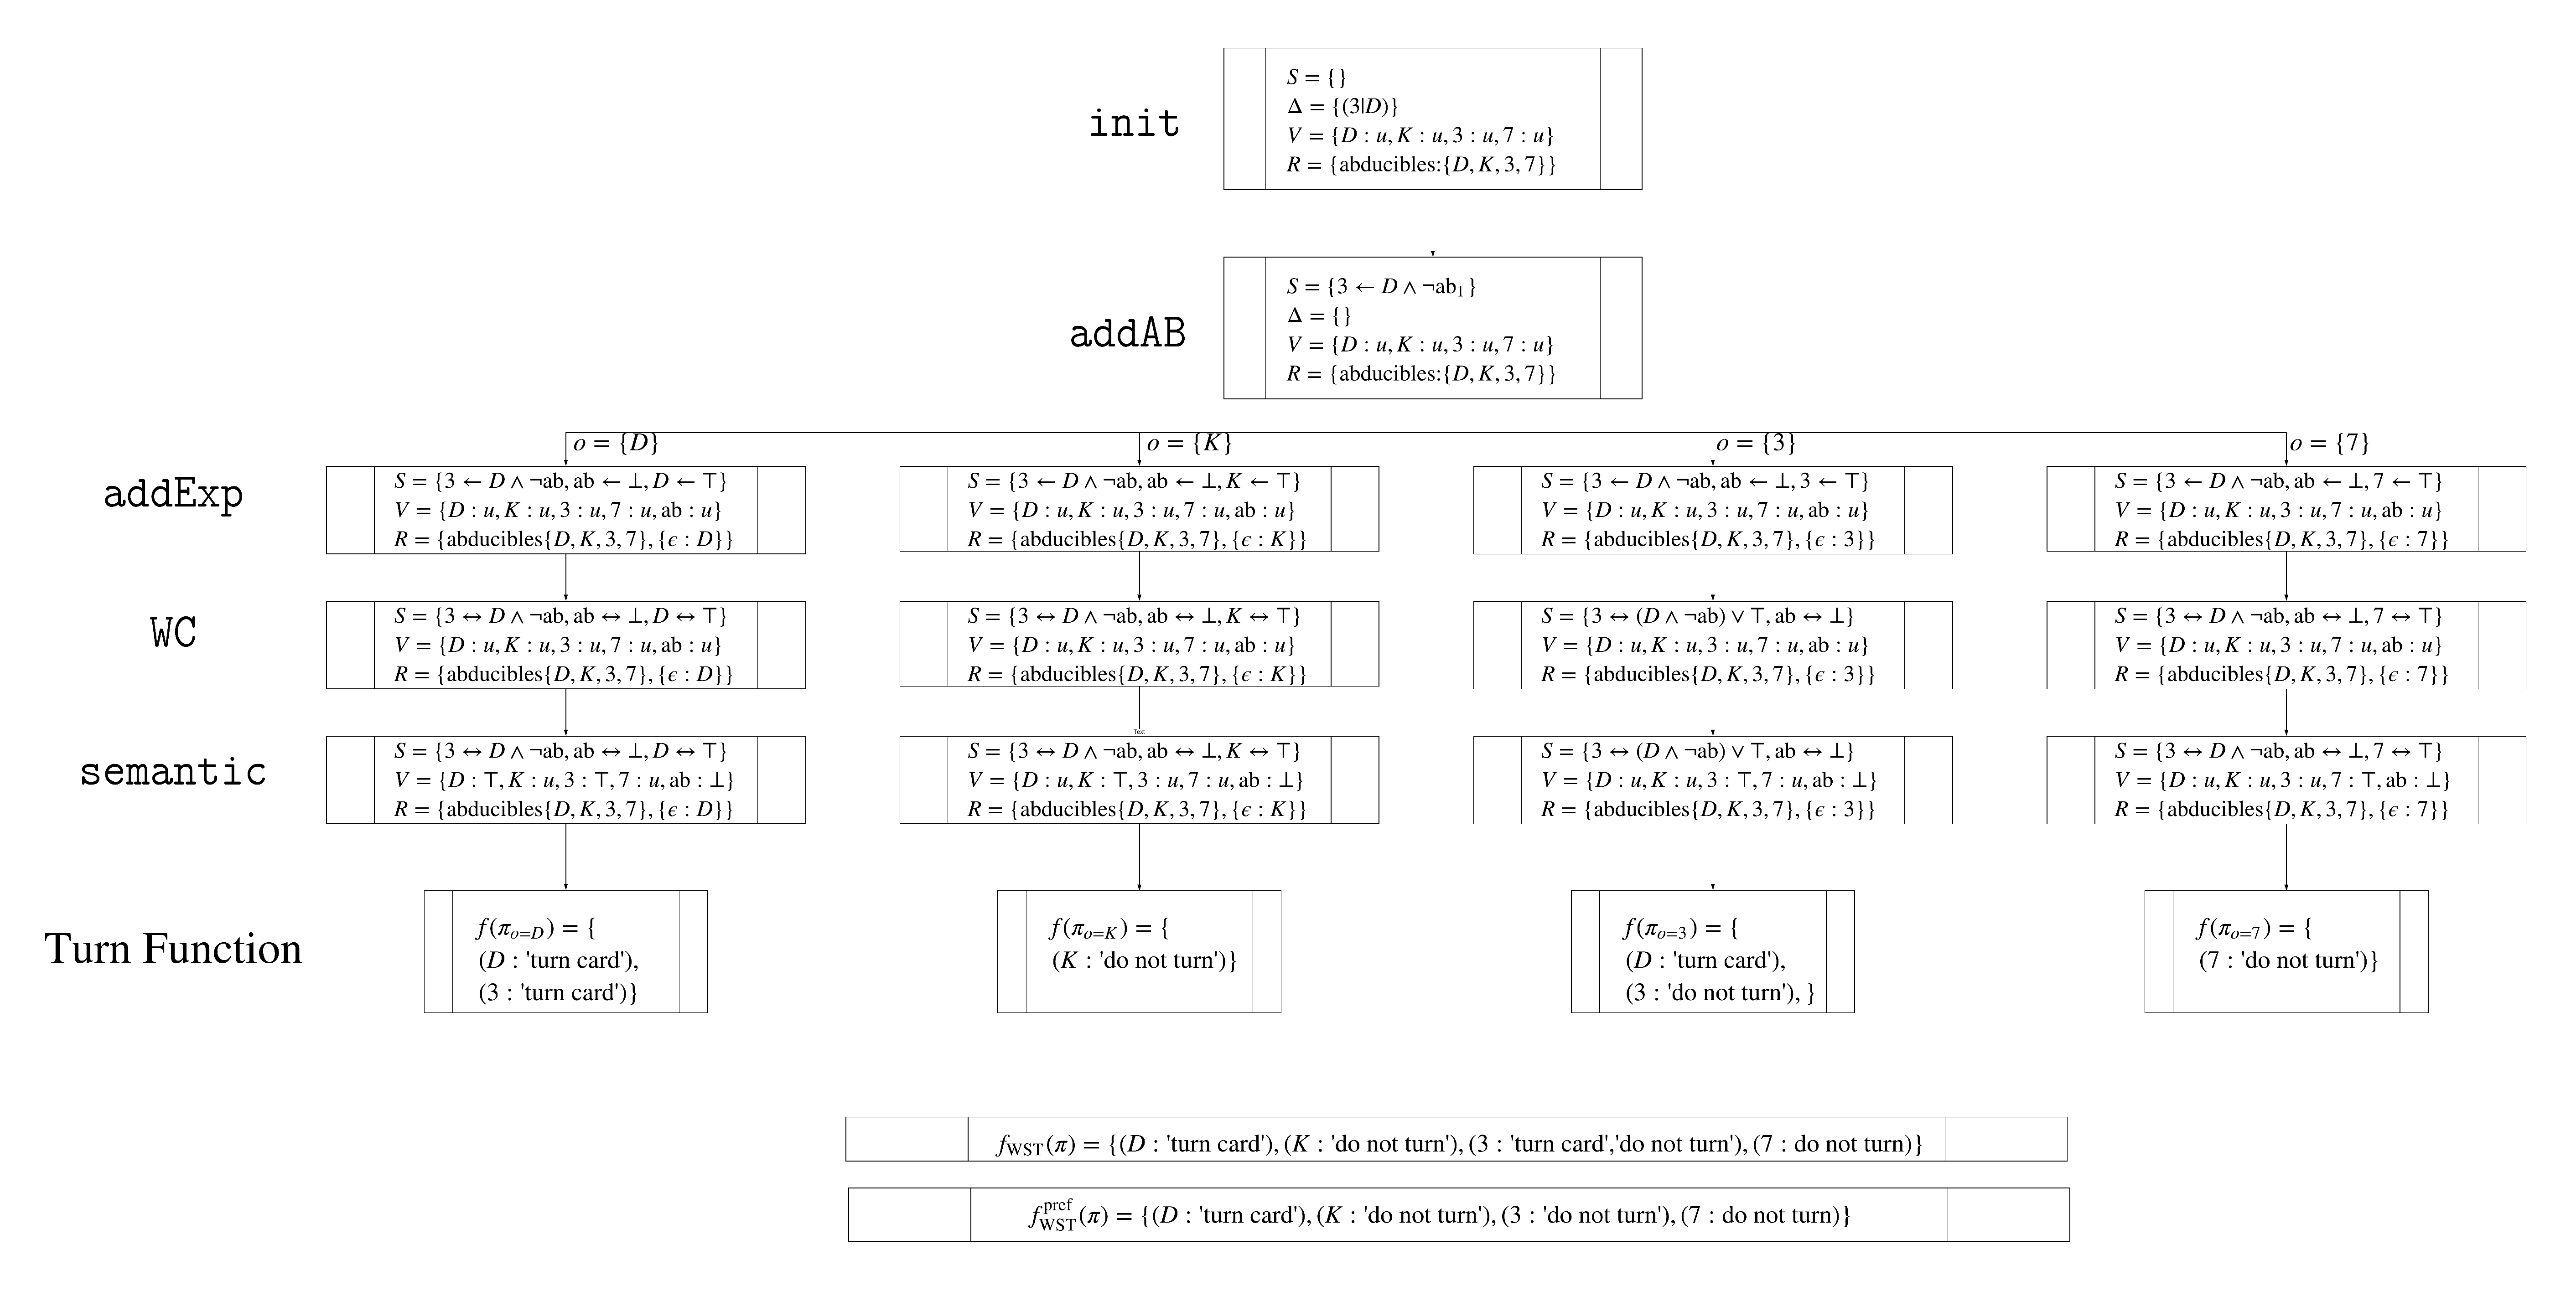
\includegraphics[width=\linewidth]{realisedSCPsWST}}
\label{fig:rSCP_WST}
\caption{Realised SCPs for the SCP interpretation of the WST $\pi_1=(s_i \longmapsto \texttt{addAB} \longmapsto \texttt{addExp}  \longmapsto \texttt{wc} \longmapsto \texttt{semantic}))$. Results mimic those observed in @TODOref's WST interpretation.}
\end{figure}

These results are not surprisingly and illustrate two important points. The first is that, for external evaluation functions that only evaluate the final epistemic state $p_n$, $f(\pi_1,O=\{o\})=f(\pi_2,O=\{o\})$ for any observation $o$. Secondly, the non-monotonic cognitive operation \texttt{addExp} means that these SCPs do not necessarily produce a single base point for $p_n$ and it will be necessary to examine the realised SCPs to determine which cards can actually be turned. Figure~\ref{fig:rSCP_WST} shows the realised SCP that can be produced for explanations of length 1 (as with @TODOcite's original WCS interpretation minimal explanations are preferred) using CTM $\pi_1$. @TODOdefineindependenceofcognitiveoperations. 

\begin{figure}
\centering{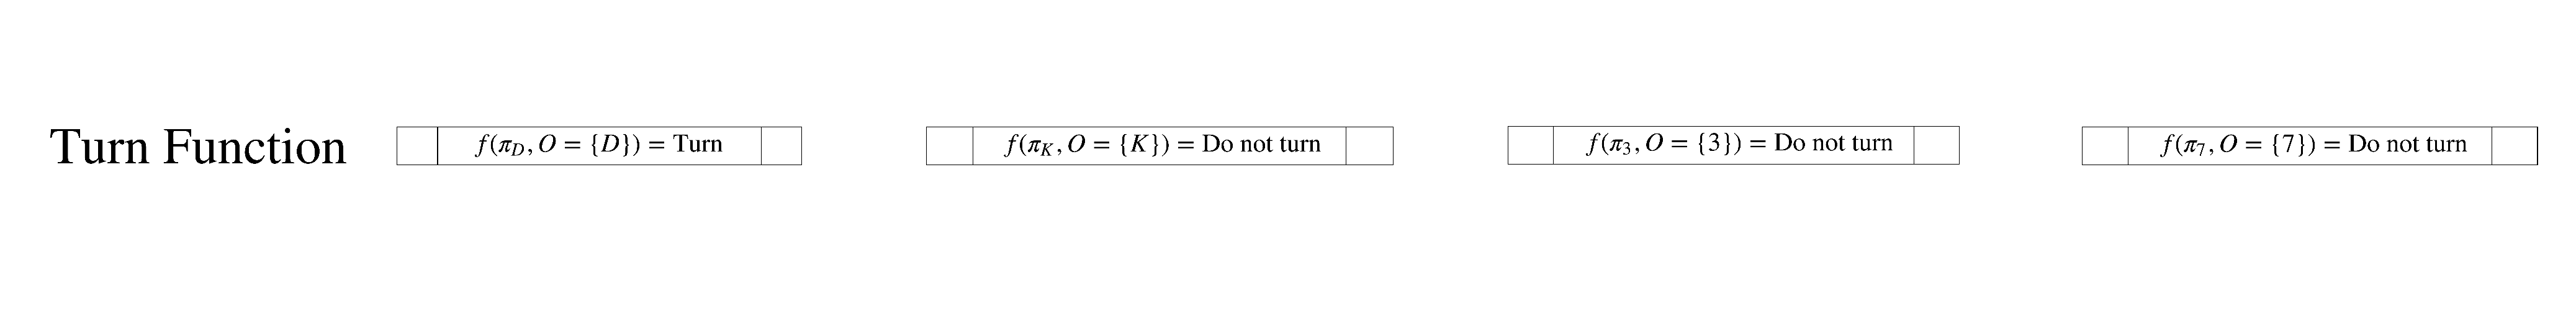
\includegraphics[width=\linewidth]{realisedSCPsWST_simple}}
\label{fig:rSCP_WST_simple}
\caption{Realised SCPs for the simplified SCP interpretation of the WST $\pi_1=(s_i \longmapsto \texttt{addAB} \texttt{addExp} \longmapsto \longmapsto \texttt{wc} \longmapsto \texttt{semantic}))$.}
\end{figure}

In order to model the three deviant cases of WST, we follow the same reasoning discussed in Section~@TODOsec and introduce two extensions to our original model: Basic Weak Completion, and Contraposition.

Basic Weak Completion is achieved by formulating a new external evaluation function $f'(\pi)=f(\pi,O=\epsilon)$. Because $I_V(\top)\models \top$, the observation is trivially satisfied and the evaluation function simply depends on whether the possible world of realised SCP assigns values which, if they were otherwise, could violate the conditional $(3|D)$. Figure~\ref{rSCP_WST_simple} illustrates $f'(r)$ for each of the realised SCPs generated in the abductive interpretation of SCPs, where the explanation $\epsilon$  is minimal.

Contraposition can be achieved by creating a new congitive operation \texttt{contra} which applies add the classical modus tolens implications to all conditionals contained in $\Delta$ of the input state.

%------
\[\texttt{contra}(\textit{input})=(\chi,e)\]
\[\chi=(\textit{input}\models (\Delta))\]
\[\Delta' := \Delta\]
\[\forall_{(\psi|\phi) \in \Delta'}\]:
\begin{itemize}
\item $S:=S \cup (\phi'\leftarrow \lnot \phi)$
\item $\Delta := \Delta\cup (\phi'| \lnot \psi)$
\item $V:=V\cup(\phi':u)$
\end{itemize}
%------



















